\subsection{多值函数}
在定义解析函数的时候,其中一个条件就是要求函数为单值的.
然而除了单值函数外,还有许多多值函数,例如对数函数和根式函数等.
碰巧的是,解析函数的许多性质仍然可以应用到多值函数上,但前提是要到
多值函数的支点 (branch points).

一般来说,多值函数$f(z)$,若$z$绕某点一周,$f(z)$不会返回原值,
我们称该点为多值函数的\textbf{支点}.若$z$绕该支点$n$周,$f(z)$复原,
则称该点为多值函数$f(z)$的$n$阶支点.
以$f(z) = z^{1/2}$为例,我们来介绍多值函数的性质.

易知,\[
    f(z) = \sqrt{r} e^{\imath \half  \Arg z}
    =  \sqrt{r} e^{\imath \left( \half \arg z + n \pi \right)},
    \]
于是,对于$n= 2k$和$n=2k+1$,$f(z)$有两个值.
\begin{equation}
    \left\{\begin{aligned}
    f_1(z) & =\sqrt{r}  e^{\imath(\arg z) / 2} \\
    f_2(z) & =-\sqrt{r}  e^{\imath(\arg z) / 2} \\
    \end{aligned}\right.
\end{equation}
这两个函数成为$f(z)= z^{1/2}$的两个\textbf{单值分支}.可以发现,
取任意包含$z=0$的闭合路径(或围道)$C$,沿着该路径绕行一圈,辐角增加$2\pi$,
可以发现$f(z)$从其一单值分支$f_1(z)$进入到另一单值分支$f_2(z)$.
若绕行两周,则回归原分支$f_1(z)$.根据定义,可知$z=0$为该函数的支点,且
为2阶支点.

此外,利用变换$z=1/t$,可以发现$z=\infty$也是2阶支点.

为了能够像对待单值函数一样对待多值函数,我们需要定义复平面Argand diagram
中的\textbf{割线}(branch cut).割线可以被认为是复平面里一个人为
设定的不可穿过的壁垒.割线的存在,使得我们能够避免形成一个包含支点的路径,
这样一来,在割线之间多值函数仍然是单值的.

对于$f(z)=z^{1/2}$,可以取任意一条过$z=0$的指向$|z|=\infty$的割线,使得
无法形成包含$z=0$支点的闭合路径.按照约定,我们通常沿着实轴或者虚轴取这样的割线.
由于割线的存在,辐角被限制在$(0,2\pi)$,因而$f(z)$保持单值.
割线的取法多种多样,正确连接各支点,同时规定辐角的值即可.

\begin{figure}[htbp]
    \centering
    
\tikzset{every picture/.style={line width=0.75pt}} %set default line width to 0.75pt        

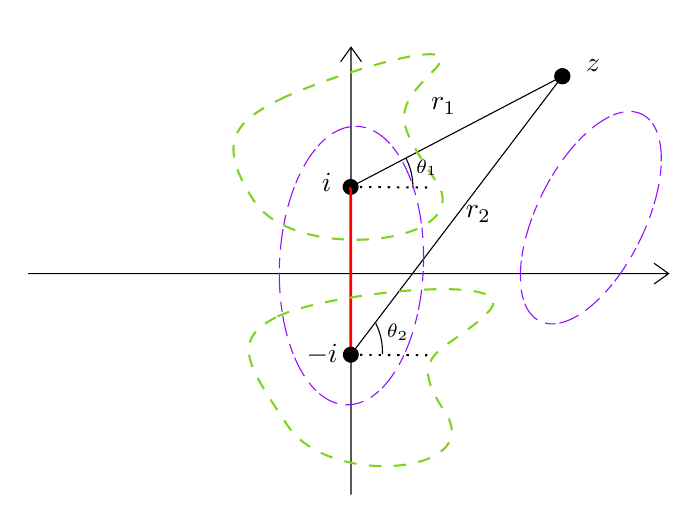
\begin{tikzpicture}[x=0.75pt,y=0.75pt,yscale=-1,xscale=1]
%uncomment if require: \path (0,300); %set diagram left start at 0, and has height of 300
% \begin{tikzpicture}[scale=1.0]

%Shape: Axis 2D [id:dp9226656499823862] 
\draw  (155.76,151.6) -- (464.29,151.6)(311.29,42.51) -- (311.29,258.08) (457.29,146.6) -- (464.29,151.6) -- (457.29,156.6) (306.29,49.51) -- (311.29,42.51) -- (316.29,49.51)  ;
%Straight Lines [id:da6217297407330797] 
\draw    (311.09,109.84) -- (413.09,56.51) ;
\draw [shift={(413.09,56.51)}, rotate = 332.4] [color={rgb, 255:red, 0; green, 0; blue, 0 }  ][fill={rgb, 255:red, 0; green, 0; blue, 0 }  ][line width=0.75]      (0, 0) circle [x radius= 3.35, y radius= 3.35]   ;
\draw [shift={(311.09,109.84)}, rotate = 332.4] [color={rgb, 255:red, 0; green, 0; blue, 0 }  ][fill={rgb, 255:red, 0; green, 0; blue, 0 }  ][line width=0.75]      (0, 0) circle [x radius= 3.35, y radius= 3.35]   ;
%Straight Lines [id:da5187482795861946] 
\draw    (311.2,190.67) -- (413.09,56.51) ;

\draw [mark = +]   (311.09,109.84) -- (311.2,190.67) [color={rgb, 255:red, 255; green, 0; blue, 0 }  ][line width=1.0];

\draw [shift={(413.09,56.51)}, rotate = 307.22] [color={rgb, 255:red, 0; green, 0; blue, 0 }  ][fill={rgb, 255:red, 0; green, 0; blue, 0 }  ][line width=0.75]      (0, 0) circle [x radius= 3.35, y radius= 3.35]   ;
\draw [shift={(311.2,190.67)}, rotate = 307.22] [color={rgb, 255:red, 0; green, 0; blue, 0 }  ][fill={rgb, 255:red, 0; green, 0; blue, 0 }  ][line width=0.75]      (0, 0) circle [x radius= 3.35, y radius= 3.35]   ;

%Straight Lines [id:da04858347938757013] 
\draw [line width=0.75]  [dash pattern={on 0.84pt off 2.51pt}]  (311.2,190.67) -- (320.53,190.73) -- (349.2,190.93) ;
%Straight Lines [id:da03323421997367659] 
\draw [line width=0.75]  [dash pattern={on 0.84pt off 2.51pt}]  (311.09,109.84) -- (333.2,110) -- (349.09,110.11) ;
%Shape: Arc [id:dp3288057226479919] 
\draw  [draw opacity=0] (337.73,96.02) .. controls (339.88,100.15) and (341.09,104.85) .. (341.09,109.84) .. controls (341.09,109.98) and (341.09,110.12) .. (341.09,110.26) -- (311.09,109.84) -- cycle ; \draw   (337.73,96.02) .. controls (339.88,100.15) and (341.09,104.85) .. (341.09,109.84) .. controls (341.09,109.98) and (341.09,110.12) .. (341.09,110.26) ;  
%Shape: Arc [id:dp0808155872490477] 
\draw  [draw opacity=0] (323.18,175.58) .. controls (325.25,179.66) and (326.43,184.28) .. (326.43,189.17) .. controls (326.43,189.55) and (326.42,189.92) .. (326.41,190.29) -- (296.43,189.17) -- cycle ; \draw   (323.18,175.58) .. controls (325.25,179.66) and (326.43,184.28) .. (326.43,189.17) .. controls (326.43,189.55) and (326.42,189.92) .. (326.41,190.29) ;  
%Shape: Polygon Curved [id:ds972117629019259] 
\draw  [color={rgb, 255:red, 126; green, 211; blue, 33 }  ,draw opacity=1 ][dash pattern={on 4.5pt off 4.5pt}][line width=0.75]  (277.2,67.6) .. controls (297.2,57.6) and (371.2,33.6) .. (351.2,53.6) .. controls (331.2,73.6) and (332.53,77.6) .. (352.53,107.6) .. controls (372.53,137.6) and (284.81,146.92) .. (264.81,116.92) .. controls (244.81,86.92) and (257.2,77.6) .. (277.2,67.6) -- cycle ;
%Shape: Polygon Curved [id:ds36093576999491384] 
\draw  [color={rgb, 255:red, 126; green, 211; blue, 33 }  ,draw opacity=1 ][dash pattern={on 4.5pt off 4.5pt}][line width=0.75]  (275.87,172.27) .. controls (298.53,160.93) and (397.2,150.27) .. (377.2,170.27) .. controls (357.2,190.27) and (336.53,188.27) .. (356.53,218.27) .. controls (376.53,248.27) and (300.81,254.92) .. (280.81,224.92) .. controls (260.81,194.92) and (253.2,183.6) .. (275.87,172.27) -- cycle ;
%Shape: Ellipse [id:dp5218651449001477] 
\draw  [color={rgb, 255:red, 144; green, 19; blue, 254 }  ,draw opacity=1 ][dash pattern={on 3.75pt off 3pt on 7.5pt off 1.5pt}] (313.49,214.35) .. controls (294.34,218.61) and (277.9,192.22) .. (276.79,155.41) .. controls (275.68,118.61) and (290.31,85.32) .. (309.47,81.07) .. controls (328.63,76.82) and (345.06,103.2) .. (346.17,140.01) .. controls (347.28,176.81) and (332.65,210.1) .. (313.49,214.35) -- cycle ;
%Shape: Ellipse [id:dp6256363959244384] 
\draw  [color={rgb, 255:red, 144; green, 19; blue, 254 }  ,draw opacity=1 ][dash pattern={on 3.75pt off 3pt on 7.5pt off 1.5pt}] (428.07,166.23) .. controls (409.33,182.7) and (393.58,177.43) .. (392.88,154.46) .. controls (392.19,131.49) and (406.82,99.52) .. (425.56,83.05) .. controls (444.3,66.58) and (460.05,71.85) .. (460.75,94.82) .. controls (461.44,117.79) and (446.81,149.76) .. (428.07,166.23) -- cycle ;


% Text Node
\draw (296,101.73) node [anchor=north west][inner sep=0.75pt]    {$i$};
% Text Node
\draw (288.67,184.4) node [anchor=north west][inner sep=0.75pt]    {$-i$};
% Text Node
\draw (423.33,47.07) node [anchor=north west][inner sep=0.75pt]    {$z$};
% Text Node
\draw (365.33,117.73) node [anchor=north west][inner sep=0.75pt]    {$r_{2}$};
% Text Node
\draw (348.67,65.73) node [anchor=north west][inner sep=0.75pt]    {$r_{1}$};
% Text Node
\draw (341.33,95.4) node [anchor=north west][inner sep=0.75pt]  [font=\scriptsize]  {$\theta _{1}$};
% Text Node
\draw (327.33,174.73) node [anchor=north west][inner sep=0.75pt]  [font=\scriptsize]  {$\theta _{2}$};


\end{tikzpicture}


    % \begin{tikzpicture}[scale=3]
    \draw[->] (-0.2,0) -- (1.2,0) node[right] {$\operatorname{Re}(z)$};
    \draw[->] (0,-0.2) -- (0,1.0) node[above] {$\operatorname{Im}(z)$};
    % \draw[dashed] (0.5,-1.5) -- (0.5,1.5);
    % \draw[dashed] (-1.5,0.5) -- (1.5,0.5);
    \draw[-latex] (1.0,0.3) -- (1.0,0.8) node[midway, right] {$\substack{\delta y\to 0\\\delta x=0}$};
    \draw[-latex] (0.3,0.8) -- (1.0,0.8) node[midway, above] {$\substack{\delta x\to 0\\\delta y=0}$};
    \filldraw [fill=none] (1,0.8) circle (0.02) node[above right] {$z_0$};
    \node at (0,0) [below left] {$O$};
\end{tikzpicture}
    \caption{对函数$f(z) = \sqrt{z^2 + 1}$的路径选取和割线示意图.}
    \label{fig:contours}
\end{figure}

\begin{example}
找出函数$f(z) = \sqrt{z^2 + 1}$的支点,并取合适的割线.
\end{example}
\begin{solution}
不难看出,
\[
  f(z) = \sqrt{z + \imath} \sqrt{z-\imath} .
\]
前面我们了解了$f(z)=\sqrt{z}$的支点为$z=0$,不难看出来,$z=\pm \imath$也会成为
该函数的两个支点.
如图\ref{fig:contours}所示,令
\[ z - i = r_1 e^{\imath \theta_1 } \quad 
    z + i = r_2 e^{\imath \theta 2}
\]
我们有\[f(z) = \sqrt{r_1 r_2} e^{\imath \half (\theta_1 + \theta_2)}.\]
如果我们做以下几种情况的闭合路径$C$,我们会得到不同的情况.若$C$
\begin{enumerate}
    \item[(i)] 不包含两个支点,那么$\theta_1 \to \theta_1, \theta_2 \to \theta_2$, 于是$f(z)\to f(z)$;
    \item[(ii)] 包含$\imath$但不含$-\imath$,那么$\theta_1 \to \theta_1 + 2\pi, \theta_2 \to \theta_2$, 于是$f(z)\to - f(z)$;
    \item[(iii)] 包含$-\imath$但不含$\imath$,那么$\theta_1 \to \theta_1, \theta_2 \to \theta_2  + 2\pi$, 于是$f(z)\to - f(z)$;
    \item[(iv)] 包含$\pm \imath$两个支点,那么$\theta_1 \to \theta_1  + 2\pi, \theta_2 \to \theta_2  + 2\pi$, 于是$f(z)\to  f(z)$.
\end{enumerate}
因此,为了阻止闭合路径绕支点完成完整的回路,我们必须选择合适的割线.图中连接$\pm \imath$的标红线段是一种选择.
\end{solution}